\section{Abläufe}

Während in Kapitel 3 die Interaktion der Hauptkomponenten \emph{Server} und der \emph{RobotUnit} abgehandelt wurden, werden im Folgenden die Abläufe der Use Cases genauer spezifiziert und auch interne Komponentenabläufe beschrieben, im speziellen die Abläufe innerhalb der \emph{RobotUnit}.
	
	\textbf{Interaktion bei Ausführung von Usecase 1 – DriveToDestionation:}\\
	Wie es schon der Name des Use Cases DriveToDestionation beschreibt, befindet sich die RobotUnit bei Ausführung diese Use Cases in einem Fahrvorgang, der vorher konkret mit der Zielposition und er Geschwindigkeit vom Server eingestellt wird. Es reagieren intern ihre Software mit der Sensor/Hardwarekomponenten, wenn ein Hindernis auftaucht und dieses mit Hilfe der durch die Sensoren gesammelten Informationen umfahren werden muss. Der unmittelbare Fahrvorgang hingegen wird über die IDrive Komponente gesteuert, die zurückmeldet wenn der Roboter das Ziel erreicht hat.
	\begin{figure}[H]
		\centering
		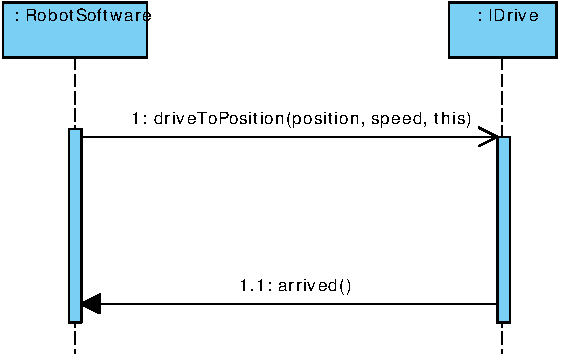
\includegraphics[width=0.75\textwidth]{img/8-driveToDest}
		\label{DriveToDestionation}
	\end{figure}
	
	
	\textbf{Interaktion bei Ausführung von Usecase 2 – Read Sensors:}\\
	In der folgenden Grafik wird der reine Anfrageprozess zwischen Server und der RobotUnit aus Kapitel 3 erweitert. Nach der Anfrage, wird der Robot alle nötigen Informationen naheinander abfragen: Sowohl die Position als auch die werden von der INorthStar Komponente zurückgeliefert. Für den Batteriestatus Orientierungsrichten muss die IBatteriekomponente angefragt werden. Erst wenn alle Informationen als Gesamtpaket bereitstehen, können sie an den Server zurückgemeldet werden.\\
	\begin{figure}[H]
		\centering
		\includegraphics[width=0.75\textwidth]{img/8-readSensors}
		\label{Read Sensors}
	\end{figure}
	
	\textbf{Interaktion bei Ausführung von Usecase 3 – Charching:}\\
	Auch beim Use Case Charching findet keine Kommunikation mit der Komponente Server statt, dafür allerdings zwischen der RobotUnit und der CharchingStation. Hat der Roboter einen bestimmten kritischen Ladestand erreicht), den er regelmäßig überprüft), läuft er die CharchingStation Komponente an. Der Ladevorgang triggert automatische, sobald der Roboter die Position der Ladestation erreich hat, und interagiert solange mit ihr bis seine Batterie wieder aufgeladen ist. Innerhalb des Robots werden zum Anfahren der Charching Station die Komponenten IBatterie mit der Position der Robotereigenen Ladestation und IDrive benötigt. Konkret: Wenn IDrive arrived() zurückgibt kann der Ladevorgang begonnen werden.\\
	\begin{figure}[H]
		\centering
		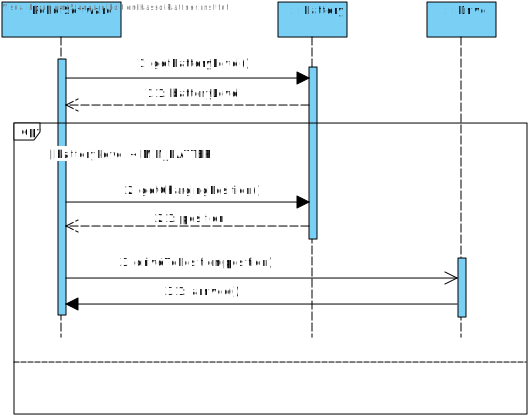
\includegraphics[width=0.75\textwidth]{img/8-charging}
		\label{Charching}
	\end{figure}
